\chapter{Introduction}
	In this course we will look at lots of methods from the domain of \emph{\ac{RL}.} \ac{RL} is an approach for agent-oriented learning where the agent learns by repeatedly acting with the environment and from rewards. Also, it does not know how the world works in advance. \ac{RL} is therefore close to how humans learn and tries to tackle the fundamental challenge of \ac{AI}:
	\begin{center}
		"The fundamental challenge in \acl{AI} and \acl{ML} is learning to make good decisions under uncertainty." (Emma Brunskill)
	\end{center}
	\ac{RL} is so general that every \ac{AI} problem can be phrased in its framework of learning by interacting. However, the typical setting is that at every time step, an agent perceives the state of the environment and chooses an action based on these perceptions. Subsequently, the agent gets a numerical reward and tries to maximize this reward by finding a suitable strategy. This procedure is illustrated in \autoref{fig:rl}.

	\section{Artificial Intelligence}
		The core question of \ac{AI} is how to build "intelligent" machines, requiring that the machine is able to adapt to its environment and handle unstructured and unseen environments. Classically, \ac{AI} was an "engine" producing answers to various queries based on rules designed by a human expert in the field. In (supervised) \ac{ML}, the rules are instead learned from a (big) data set and the "engine" produces answers based on the data. However, this approach (leaning from labeled data) is not sufficient for \ac{RL} as demonstrations might be imperfect, the correspondence problem, and that we cannot demonstrate everything. We can break these issues down as follows: supervised learning does not allow "interventions" (trial-and-error) and evaluative feedback (reward).

		The core idea leading to \ac{RL} was to not program machines to simulate an adult brain, but to simulate a child's brain that is still learning. \ac{RL} formalizes this idea of intelligence to interpret rich sensory input and choosing complex actions. We know that this may be possible as us humans do it all the time. This lead to the \ac{RL} view on \ac{AI} depicted in \autoref{fig:rl} and is based on the hypothesis that learning from a scalar reward is sufficient to yield intelligent behavior (Sutton and Barto, 2018).

		\begin{figure}
			\centering
			\begin{tikzpicture}[->, cmp/.style = { draw, rectangle, minimum width = 2.5cm, minimum height = 0.75cm }]
				\node [cmp] (agent) {Agent};
				\node [cmp, right = 2 of agent] (env) {Environment};
				\coordinate [above = 0.5 of agent] (a);
				\coordinate [above = 0.5 of env] (b);

				\coordinate [left = 0.5 of agent.south] (agentL);
				\coordinate [right = 0.5 of agent.south] (agentR);
				\coordinate [below = 1.25 of agentL] (fL);
				\coordinate [below = 0.50 of agentR] (fR);

				\coordinate [left = 0.5 of env.south] (envL);
				\coordinate [right = 0.5 of env.south] (envR);
				\coordinate [below = 0.50 of envL] (eL);
				\coordinate [below = 1.25 of envR] (eR);

				\draw (agent) to (a) to node[above]{Action \(a_t\)} (b) to (env);
				\draw (envL) to (eL) to node[below]{Reward \( r_t \gets r_{t + 1} \)} (fR) to (agentR);
				\draw (envR) to (eR) to node[below]{State \( s_t \gets s_{t + 1} \)} (fL) to (agentL);
			\end{tikzpicture}
			\caption{The Reinforcement Learning Cycle}
			\label{fig:rl}
		\end{figure}
	% end

	\section{Reinforcement Learning Formulation}
		\ac{RL} tries to \emph{maximize the long-term reward} by finding a strategy/policy with the general assumption that it is easier to assess a behavior by specifying a cost than specifying the behavior directly. In general, we have the following things different to most (un)supervised settings:
		\begin{itemize}
			\item no supervision, but only a reward signal
			\item feedback (reward) is always delayed and not instantaneous
			\item time matters, the data is sequential and by no means i.i.d.
			\item the agent's actions influence the subsequent data, i.e., the agent generates its own data
		\end{itemize}
		In addition to this, \ac{RL} is challenged by a numerous complicated factors and issues, e.g., dynamic state-dependent environments, stochastic and unknown dynamics and rewards, exploration vs. exploitation, delayed rewards (how to assign a temporal credit), and very complicated systems (large state spaces with unstructured dynamics). For designing an \ac{RL}-application, we usually have to choose the state representation, decide how much prior knowledge we want to put into the agent, choose an algorithm for learning, design an objective function, and finally decide how we evaluate the resulting agent. By all these decisions, we want to reach a variety of goals, e.g., convergence, consistency, good generalization abilities, high learning speed (performance), safety, and stability. However, we are usually pretty restricted in terms of computation time, available data, restrictions in the way we act (e.g., safety constraints), and online vs. offline learning.

		This sounds like a lot and, in fact, is! We therefore often limit ourselves onto specific (probably simpler) sub-problems and solve them efficiently under some assumptions. Some common flavors of the \ac{RL} problem are, for instance:
		\begin{itemize}
			\item \emph{Full:} no additional assumptions, the agent can only probe the environment through the state dynamics and its actions; the agent has to understand the environment
			\item \emph{Filtered State and Sufficient Statistics:} assumption of a local Markov property (i.e., the next state only depends on the current state and action, and not on the past), decomposable rewards (into specific time steps); we can show that every problem is a (probably infinite) instance of this assumption, but how to filter the state to get such properties?
			\item \emph{Markovian Observable State:} assume that we can observe the state fulfilling the Markov property directly
			\item \emph{Further Simplifications:} contextual bandits (the dynamics do not depend on the action or the past and current state at all); bandits (only a single state)
		\end{itemize}
		We can summarize the different \ac{RL}-like problems in a matrix, see \autoref{tab:problemClassification}.

		\begin{table}
			\centering
			\begin{tabular}{c||cc}
				\toprule
				            & actions \emph{do not} change the state of the world & actions change the state of the world \\ \midrule
				 no model   &                (Multi-Armed) Bandits                &        Reinforcement Learning         \\
				known model &                   Decision Theory                   &       Optimal Control, Planning       \\ \bottomrule
			\end{tabular}
			\caption{Problem Classification}
			\label{tab:problemClassification}
		\end{table}

		\subsection{Components}
			To solve an \ac{RL} problem, we need three ingredients:
			\begin{enumerate}
				\item Model Learning
					\begin{itemize}
						\item we want to approximate and learn the state transfer using methods from supervised learning
						\item need to generate actions for model identification
						\item estimation of the model or the model's parameters
					\end{itemize}
				\item Optimal Control/Planning
					\begin{itemize}
						\item generation of optimal control inputs
					\end{itemize}
				\item Performance Evaluation
			\end{enumerate}
		% end
	% end

	\section{Wrap-Up}
		\begin{itemize}
			\item why \ac{RL} is crucial for \ac{AI} and why all other approaches are ultimately doomed
			\item background and characteristics of \ac{RL}
			\item classification of \ac{RL} problems
			\item core components of \ac{RL} algorithms
		\end{itemize}
		% TODO: Sutton, Chapter 1
	% end
% end

\chapter{Preliminaries}
	In this chapter we cover some preliminaries that are necessary for understanding the rest of the course. Note that most of this content is dense and should be used as a reference throughout this course as oppose to an actual introduction to the topic.

	\section{Functional Analysis}
		\begin{definition}[Normed Vector Space]
			A \emph{normed vector space} is a vector space \(\mathcal{X}\) over \(X\) equipped with a \emph{norm} \( \lVert \cdot \rVert : \mathcal{X} \to \R \) that has the following properties:
			\begin{enumerate}
				\item \( \lVert x \rVert \geq 0 \) for all \( x \in \mathcal{X} \) and \( \lVert x \rVert = 0 \) iff \( x = 0 \) (non-negativity)
				\item \( \lVert \alpha x \rVert = \lvert \alpha \rvert \lVert x \rVert \) for all \( \alpha \in X \) and \( x \in \mathcal{X} \) (homogenity)
				\item \( \lVert x_1 + x_2 \rVert \leq \lVert x_1 \rVert + \lVert x_2 \rVert \) for all \( x_1, x_2 \in \mathcal{X} \) (triangle inequality)
			\end{enumerate}
		\end{definition}
		For the rest of this course we usually use real finite-dimensional vectors spaces \( \mathcal{X} = \R^d \), \( d \in \N^+ \), the \(L_\infty\)-norm \( \lVert \cdot \rVert_\infty \), and (weighted) \(L_2\)-norms \( \lVert \cdot \rVert_{2, \rho} \).

		\begin{definition}[Complete Vector Space]
			A vector space \(\mathcal{X}\) is \emph{complete} if every Cauchy sequence\footnote{This section is already overflowing with mathematical rigor compared to the rest of the course, so we will skip the definition of a Cauchy sequence here.} in \(\mathcal{X}\) has a limit in \(\mathcal{X}\).
		\end{definition}

		\begin{definition}[Contraction Mapping]
			Let \(\mathcal{X}\) be a vector space equipped with a norm \(\lVert \cdot \rVert\). An operator \( T : \mathcal{X} \to \mathcal{X} \) is called an \emph{\(\alpha\)-contraction mapping} if \( \exists \alpha \in [0, 1) : \forall x_1, x_2 \in \mathcal{X} : \lVert T x_1 - T x_2 \rVert \leq \alpha \lVert x_1 - x_2 \rVert \). If only \( \exists \alpha \in [0, 1] : \forall x_1, x_2 \in \mathcal{X} : \lVert T x_1 - T x_2 \rVert \leq \alpha \lVert x_1 - x_2 \rVert \), \(T\) is called \emph{non-expanding.}
		\end{definition}

		\begin{definition}[Lipschitz Continuity]
			Let \(\mathcal{X}\) and \(\mathcal{Y}\) be vector spaces equipped with norms \(\lVert \cdot \rVert_X\) and \(\lVert \cdot \rVert_Y\), respectively. A function \( f : \mathcal{X} \to \mathcal{Y} \) is called \emph{Lipschitz-continuous} if \( \exists L \geq 0 : \forall x_1, x_2 \in \mathcal{Y} : \lVert f(x_1) - f(x_2) \rVert_Y \leq L \lVert x_1 - x_2 \rVert_X \).
		\end{definition}

		\begin{remark}
			Obviously, every contraction mapping is also Lipschitz-continuous with Lipschitz-constant \(L \triangleq \alpha\) and is therefore continuous. Also, the product of two Lipschitz-continuous mappings is Lipschitz-continuous and therefore \(T^n = T \circ \dots \circ T\) is Lipschitz-continuous, too.
		\end{remark}

		\begin{definition}[Fixed Point]
			Let \(\mathcal{X}\) be a vector space equipped and let \( T : \mathcal{X} \to \mathcal{X} \) be an operator. Then \(x \in \mathcal{X}\) is a \emph{fixed point} of \(T\) if \( T x = x \).
		\end{definition}

		\begin{theorem}[Banach Fixed Point Theorem]
			Let \(\mathcal{X}\) be a complete vector space with a norm \(\lVert \cdot \rVert\) and let \( T : \mathcal{X} \to \mathcal{X} \) be an \(\alpha\)-contraction mapping. Then \(T\) has a unique fixed point \(x^\ast \in \mathcal{X}\) and for all \(x_0 \in \mathcal{X}\) the sequence \( x_{n + 1} = T x_n \) converges to \(x^\ast\) geometrically, i.e., \( \lVert x_n - x^\ast \rVert \leq \alpha^n \lVert x_0 - x^\ast \rVert \).
		\end{theorem}
	% end

	\section{Statistics}
		This section introduces some concepts of statistics, but you should

		\subsection{Monte-Carlo Estimation}
			Let \(X\) be a random variable with mean \( \mu = \E[X] \) and variance \( \sigma^2 = \Var[X] \) and let \( \{ x_i \}_{i = 1}^{n} \) be i.i.d. realizations of \(X\). We then have the \emph{empirical mean} \( \hat{\mu}_n = \frac{1}{n} \sum_{i = 1}^{n} x_i \) and we can show that \( \E[\hat{\mu}_n] = \mu \) and \( \Var[\hat{\mu}_n] = \sigma^2/n \). Also, if the sample size \(n\) goes to infinity, we have the \emph{strong} and \emph{weak law of large numbers,} respectively:
			\begin{align}
				P\bigl( \lim\limits_{n \to \infty} \hat{\mu}_n = \mu \bigr) &= 1 &
				\lim\limits_{n \to \infty} P\bigl( \lvert \hat{\mu}_n - \mu \rvert > \epsilon \bigr) &= 0
			\end{align}
			Also, we have the \emph{central limit theorem:} no matter the distribution of \(P\), its mean value converges to a normal distribution, \( \sqrt{n} (\hat{\mu}_n - \mu) \overset{D}{\to} \mathcal{N}(0, \sigma^2) \).
		% end

		\subsection{Bias-Variance Trade-Off}
			When evaluating/training a \ac{ML} model, the error is due to two factors (illustrated in \autoref{fig:biasVariance}):
			\begin{itemize}
				\item \emph{bias,} i.e., the distance to the expected prediction
				\item \emph{variance,} i.e., the variability of a prediction for a given data point
			\end{itemize}
			In general, we want to minimize both, but we can only minimize one of them! This is known as the \emph{bias-variance trade-off.}

			\begin{figure}
				\centering
				\begin{subfigure}{0.3\linewidth}
					\centering
					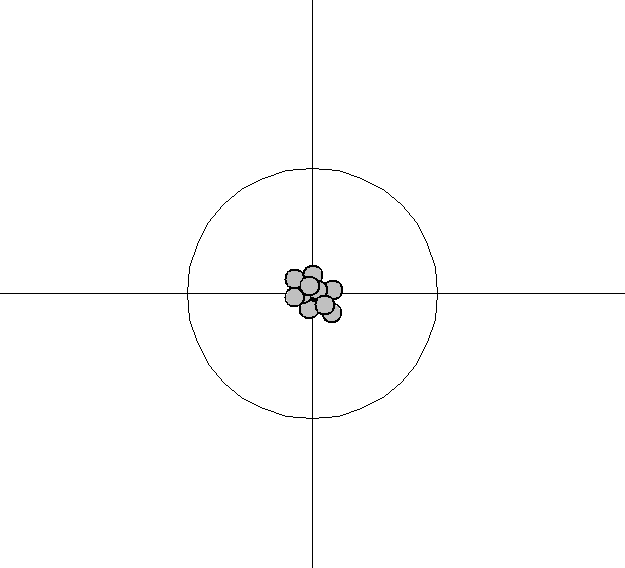
\includegraphics[width=\linewidth]{figures/low-bias-low-variance}
					\caption{Low Bias, Low Variance}
				\end{subfigure}
				~
				\begin{subfigure}{0.3\linewidth}
					\centering
					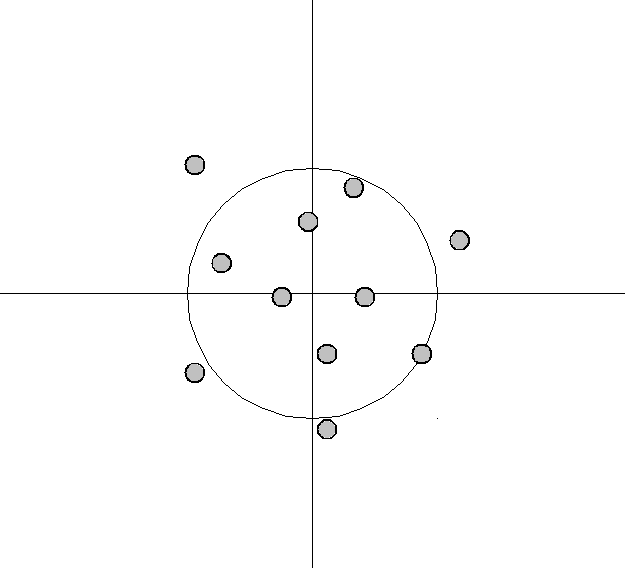
\includegraphics[width=\linewidth]{figures/low-bias-high-variance}
					\caption{Low Bias, High Variance}
				\end{subfigure}
				\\[5pt]
				\begin{subfigure}{0.3\linewidth}
					\centering
					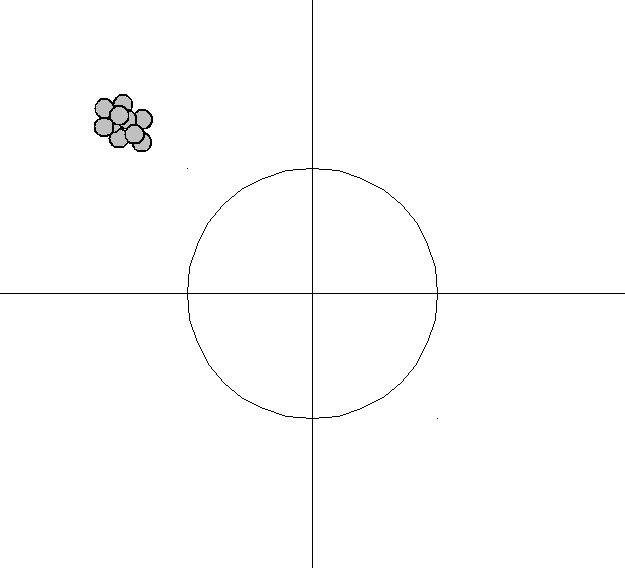
\includegraphics[width=\linewidth]{figures/high-bias-low-variance}
					\caption{High Bias, Low Variance}
				\end{subfigure}
				~
				\begin{subfigure}{0.3\linewidth}
					\centering
					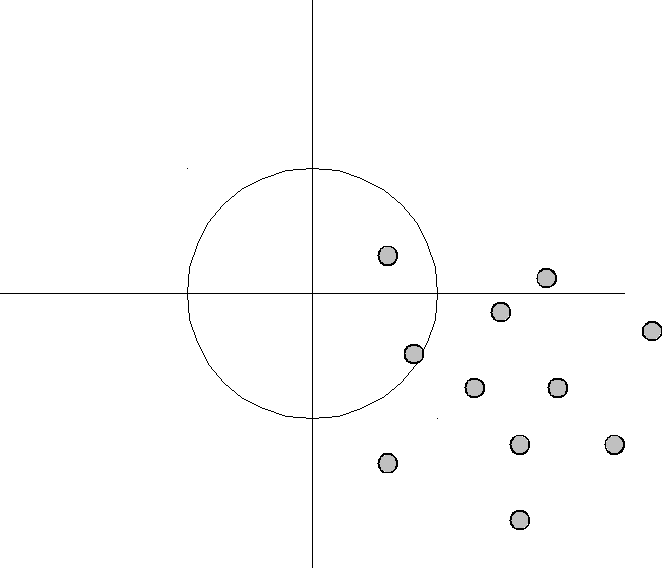
\includegraphics[width=\linewidth]{figures/high-bias-high-variance}
					\caption{High Bias, High Variance}
				\end{subfigure}
				\caption[Bias-Variance Trade-Off]{Bias-Variance Trade-Off; Source: Bernhard Thiery (CC BY-SA 3.0)}
				\label{fig:biasVariance}
			\end{figure}
		% end

		\subsection{Important Sampling}
			If we want to estimate the expectation of some function \(f(x)\) for \( x \sim p(x) \), but cannot sample from \(p(x)\) (which is often the case for complicated models), we can instead use the following relation(s):
			\begin{gather}
				\E_{x \sim p}\bigl[ f(x) \bigr]
					= \sum_x f(x) p(x)
					= \sum_x f(x) \frac{p(x)}{q(x)} q(x)
					= \E_{x \sim q} \biggl[ f(x) \frac{p(x)}{q(x)} \biggr] \\
				\E_{x \sim p}\bigl[ f(x) \bigr]
					= \int\! f(x) p(x) \dd{x}
					= \int\! f(x) \frac{p(x)}{q(x)} p(x) \dd{x}
					= \E_{x \sim q} \biggl[ f(x) \frac{p(x)}{q(x)} \biggr]
			\end{gather}
			and sample from a surrogate distribution \(q(x)\). This approach obviously has problems if \(q\) does not cover \(p\) sufficiently well along with other problems. See Bishop, 2006, Chapter 11 for details.
		% end

		\subsection{Linear Function Approximation}
			A basic approximator we will need often is the linear function approximator \( f(\vec{x}) = \vec{w}^\transposed \vec{\phi}(\vec{x}) \) with weights \(\vec{w}\) and features \(\vec{\phi}(\vec{x})\). As the weights are optimized and the features are designed, we have lots of variability here. Actually, constructing useful features is the influential step on the approximation quality. Most importantly, features are the only point where we can introduce interactions between different dimensions. A good representations therefore captures all dimensions and all (possibly complex) interaction.

			We will now go over some frequently used features.

			\paragraph{Polynomial Features}
				\emph{Polynomial features} are particularly simple and capture the interaction between dimensions by multiplication. For instance, the first- and second-order polynomial features of a two-dimensional state \( \vec{x} = (x_1, x_2)^\transposed \) are:
				\begin{align}
					\vec{\phi}_\mathit{P1}(\vec{x}) &= (1, x_1, x_2, x_1 x_2)^\transposed &
					\vec{\phi}_\mathit{P2}(\vec{x}) &= (1, x_1, x_2, x_1 x_2, x_1^2, x_2^2, x_1 x_2^2, x_1^2 x_2, x_1^2, x_2^2)
				\end{align}
				However, the number of features grows \emph{exponentially} with the dimension!
			% end

			\paragraph{Fourier Basis}
				Fourier series can be used to approximate periodic functions by adding sine and cosine waves with different frequencies and amplitudes. Similarly, we can use them for general function approximation of functions with bounded domain. As it is possible to approximate any even function with just cosine waves and we are only interested in bounded domains, we can set this domain to positive numbers only and can therefore approximate any function. For one dimension, the \(n\)-th order \emph{Fourier (cosine) basis} is
				\begin{equation}
					\phi_m(x) = \cos(\pi m \tilde{x}),\quad m = 0, 1, \dots, n.
				\end{equation}
				and \( \tilde{x} \) is a normalized version of \(x\), i.e., \( \tilde{x} = (x - x_\mathrm{max}) / (x_\mathrm{max} - x_\mathrm{min}) \).
			% end

			\paragraph{Coarse Coding}
				\emph{Coarse coding} divides the space into \(M\) different regions and produced \(M\)-dimensional coding features for which the \(j\)-th entry is \num{1} iff the data point lies withing the respective region; all values the data point does not lie in are \num{0}. Features with this codomain are also called \emph{sparse.}
			% end

			\paragraph{Tile Coding}
				\emph{Tile coding} is a computationally efficient form of coarse coding which use square \emph{tilings} of space. It uses \(N\) tilings, each composed of \(M\) tiles. The features "vector" is then an \(N \times M\) matrix where a single value is \num{1} iff \(x\) lies inside the tile and \num{0} otherwise. \autoref{fig:tileCoding} shows an illustration of this coding.

				\begin{figure}
					\centering
					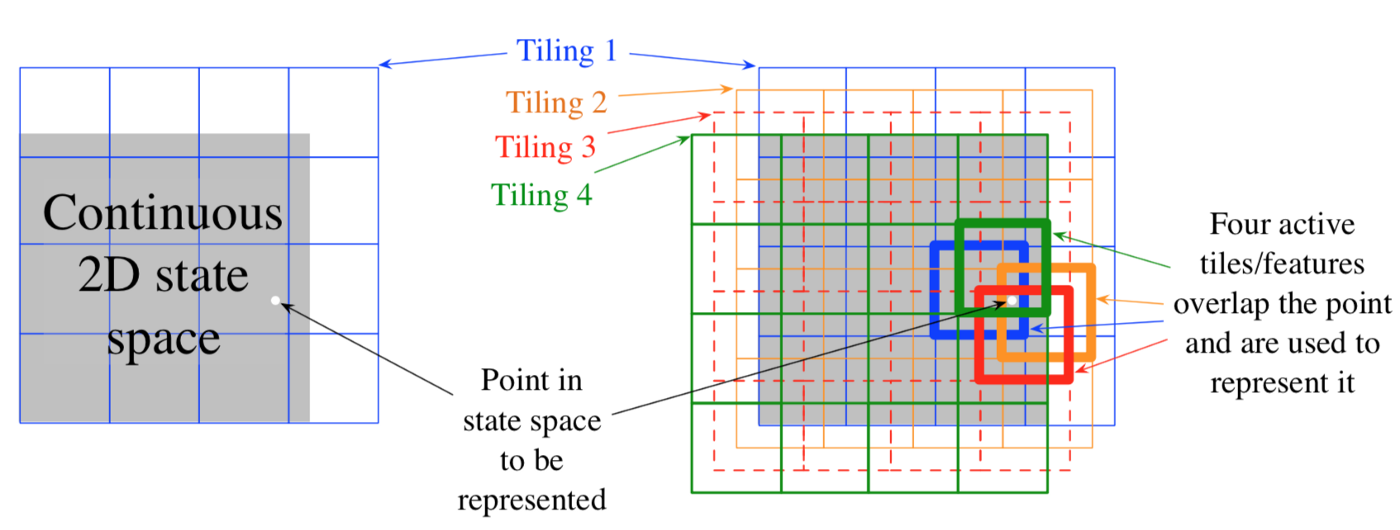
\includegraphics[width=0.9\linewidth]{figures/tile-coding}
					\caption[Tile Coding]{Tile Coding; Source: {\small \url{https://towardsdatascience.com/reinforcement-learning-tile-coding-implementation-7974b600762b}}}
					\label{fig:tileCoding}
				\end{figure}
			% end

			\paragraph{Radial Basis Functions}
				\emph{Radial basis functions (\acsp{RBF}\acused{RBF})} are a generalization of coarse coding where the features are in the interval \((0, 1]\). A typical \ac{RBF} is the Gaussian
				\begin{equation}
					\phi_j(\vec{x}) = \exp\Biggl\{ -\frac{\lVert \vec{x} - \vec{c}_j \rVert_2^2}{2 \sigma_j^2} \Biggr\}
				\end{equation}
				with center \(\vec{c}_j\) and bandwidth \( \sigma_j^2 \).
			% end

			\paragraph{Neural Networks}
				A very powerful alternative to hand-crafting features are \emph{\aclp{NN} (\acsp{NN}\acused{NN}).} By stacking multiple layers of learned features, they are very powerful prediction machines.
			% end
		% end

		\subsection{Likelihood-Ratio Trick}
			Suppose we need to differentiate the expectation of some function \( f(x) \) w.r.t. \(\theta\) where \( x \sim p_\theta(\cdot) \). However, we cannot directly calculate \( \E_{x \sim p_\theta}[f(x)] \) or "differentiate through sampling." Instead, we can use the identity
			\begin{equation}
				\dv{z} \log h(z) = \frac{h'(z)}{h(z)}
				\qquad\implies\qquad
				f'(z) = h(z) \, \dv{z} \log h(z)
			\end{equation}
			to reformulate the derivative of the expectation as
			\begin{equation}
				\pdv{\theta} \E_{x \sim p_\theta}[f(x)]
					= \int\! f(x) \pdv{\theta} p_\theta(x) \dd{x}
					= \int\! f(x) \biggl( \pdv{\theta} p_\theta(x) \biggr) p_\theta(x) \dd{x}
					= \E_{x \sim p_\theta} \biggl[ f(x) \, \pdv{\theta} p_\theta(x) \biggr].
			\end{equation}
			While this is a very powerful approach, the gradient estimator exhibits high variance!
		% end

		\subsection{Reparametrization Trick}
			Suppose we need to differentiate the expectation of some function \( f(x) \) w.r.t. \(\theta\) where \( x \sim p_\theta(\cdot) \). However, we cannot directly calculate \( \E_{x \sim p_\theta}[f(x)] \) or "differentiate through sampling." Instead, we reformulate the expectation with a function \( x = g_\theta(\varepsilon) \) that separates the random components \(\varepsilon\) from the deterministic ones \(\theta\) such that we can reparameterize the expectation as
			\begin{equation}
				\E_{x \sim p_\theta}[f(x)] = \E_\varepsilon\bigl[ f\bigl( g_\theta(\varepsilon) \bigr) \bigr].
			\end{equation}
			For instance, if \( p_\theta(x) = \mathcal{N}(\mu_\theta, \sigma_\theta^2) \) is a Gaussian, \( g_\theta(\varepsilon) = \mu_\theta + \sigma_\theta \varepsilon \) with \( \varepsilon \sim \mathcal{N}(0, 1) \). We can now simply use the chain rule to take the derivative w.r.t. \(\theta\). Compared to the likelihood-ratio trick, this estimator has less variance!
		% end
	% end

	\section{Miscellaneous}
		Finally, this section contains all the stuff that does not fit into the categories before.

		\subsection{Useful Integrals}
			The following hold for a distribution \( p_\theta(x) \):
			\begin{align}
				\int\! \pdv{\theta} p_\theta(x) \dd{x} &= 0 &
				\int\! \pdv{\theta} \log p_\theta(x) \dd{x} &= \int\! \frac{\pdv{\theta} p_\theta(x)}{p_\theta(x)} \dd{x} = 0
			\end{align}
			The first identity can be shown by swapping the integral and derivative and using the normalization condition of probability densities. For the second we use integration by parts with \( f' = \pdv{\theta} p_\theta(x) \), for which \(f = 0\) due to the first integral. Hence, the second follows.
		% end
	% end
% end

\chapter{Markov Decision Processes and Policies}
	In this chapter we will develop the groundwork for all upcoming chapters and define some important mathematical concepts.

	\section{Markov Decision Processes}
		A \emph{\ac{MDP}} describes the environment for \ac{RL} \emph{formally} for the case where we can fully observe the environment, i.e., we directly "see" the state. Also, the current state fully characterized the system and future states are independent from the past \emph{(Markov property).} This mathematical framework allows precision and rigorous reasoning on, for instance, optimal solutions and convergence (note, however, that we will only touch the tip of the iceberg in theoretical analysis and we will be less rigorous than some mathematician may wish). The nice this of \acp{MDP} is there wide applicability: we can frame almost all \ac{RL} problems as \acp{MDP}. Most of the remaining chapter here focuses on fully observable and finite \acp{MDP}, i.e., the number of states and actions is finite. \autoref{tab:markovModels} shows an overview over different Markov models.

		We now went over some mathematical definitions for building up the "Markovian framework."

		\begin{table}
			\centering
			\begin{tabular}{c|cc}
				\toprule
				                  & \multicolumn{2}{c}{\textbf{All states observable?}} \\
				\textbf{Actions?} &           Yes           &            No             \\ \midrule
				       Yes        & Markov Decision Process & Partially Observable MDP  \\
				       No         &      Markov Chain       &    Hidden Markov Model    \\ \bottomrule
			\end{tabular}
			\caption{Types of Markov Models}
			\label{tab:markovModels}
		\end{table}

		\begin{definition}[Markov Property]
			A stochastic process \(X_t\) is \emph{Markovian} or \emph{fulfills the Markov property} if \( P_t(S_{t + 1} = s' \given S_t = s, S_{t - 1} = k_{t - 1}, \dots, S_0 = k_0) = P_t(S_{t + 1} = s' \given S_t = s) \) for all \(t\).
		\end{definition}

		\begin{definition}[Stationary Transition Probabilities]
			If \( P_t(S_{t + 1} = s' \given S_t = s) \) is time invariant, \( p_{ss'} \coloneqq P_t(S_{t + 1} = s' \given S_t = s) \) are the \emph{stationary transition probabilities.}
		\end{definition}

		\begin{definition}[State Transition Matrix]
			With the transition probabilities \(p_{ss'}\), let \( \mat{P}_{ss'} \coloneqq p_{ss'} \) for all \(s\), \(s'\) be the \emph{transition matrix.}
		\end{definition}

		\begin{definition}[Markov Chain]
			A \emph{Markov chain} is a tuple \( \langle \mathcal{S}, \mat{P}, \iota \rangle \) with the (finite) set of discrete-time states \(S_t \in \mathcal{S}\), \( n \coloneqq \lvert \mathcal{S} \rvert \), transition matrix \( \mat{P} \in [0, 1]^{n \times n} \), and the initial state distribution \( \iota_i = P(S_0 = i) \).
		\end{definition}

		\begin{definition}[Probability Row Vector]  \label{def:probRowVector}
			The vector \( \vec{p}_t \coloneqq \sum_{i = 1}^{n} P(S_t = i) \vec{e}_i^\transposed \) with the \(i\)-th unit vector \(\vec{e}_i\) and includes the probability of being in the \(i\)-th state at time step \(t\).
		\end{definition}

		\begin{theorem}[Chapman-Kolmogorov for Finite Markov Chains]
			The probability row vector \( \vec{p}_{t + k} \) at time step \(t + k\) starting from \(\vec{p}_t\) at time step \(t\) is given by \( \vec{p}_{t + k} = \vec{p}_t \mat{P}^k \).
		\end{theorem}
		\begin{proof}
			Assume w.l.o.g. \( t = 0 \) We proof this by induction. For the base case, let \(k = 1\). Let \( \vec{p}_0 = (p_{0, 1}, p_{0, 2}, \dots, p_{0, n}) \) be an arbitrary probability row vector. By linearity, we have
			\begin{align}
				\vec{p}_0 \mat{P}_{ss'}
					&= \sum_{i = 1}^{n} p_{0, 1} \vec{e}_i^\transposed \mat{P}
					 = \sum_{i = 1}^{n} p_{0, 1} \mat{P}_i \\
				\intertext{where \(\mat{P}_i\) is the \(i\)-th row of \(\mat{P}\). Rewriting this equation in terms of explicit transition probabilities, we have}
					&= \sum_{i = 1}^{n} P(S_0 = i) \sum_{j = 1}^{n} \vec{e}_j^\transposed P(S_1 = j \given S_0 = i)
					 = \sum_{j = 1}^{n} \vec{e}_j^\transposed \,\sum_{i = 1}^{n} P(S_0 = i) P(S_1 = j \given S_0 = i) \\
					&= \sum_{j = 1}^{n} \vec{e}_j^\transposed \,\sum_{i = 1}^{n} P(S_1 = j, S_0 = i)
					 = \sum_{j = 1}^{n} \vec{e}_j^\transposed P(S_1 = j)
					 = \sum_{j = 1}^{n} p_{1, j} \vec{e}_j^\transposed
					 = \vec{p}_1.
			\end{align}
			The first equality is due to the definition of \(\mat{P}_i\), the third is due to the definition of conditional probabilities, the fourth is due to marginalizing out \(S_0\), and the final is just another application of the definit ion of the probability row vector. For the induction step \( k \to k + 1 \), assume that \( \vec{p}_k = \vec{p}_t \mat{P}^k \) holds for some \(k\). We then have \( \vec{p}_{k + 1} = \vec{p}_k \mat{P} = \vec{p}_0 \mat{P}^k \mat{P} = \vec{p}_0 \mat{P}^{k + 1} \) where the first equality is due to the base case and the second is due to the induction hypothesis.
		\end{proof}

		\begin{definition}[Steady State]
			A probability row vector \(\vec{p}\) is called a \emph{steady} state if an application of the transition matrix does not change it, i.e., \( \vec{p} = \vec{p} \mat{P} \).
		\end{definition}
		\begin{remark}
			While the steady state is in general not independent of the initial state (consider, for instance, \( \mat{P} = \mat{I} \)), it gives insights in which states of the Markov chain are visited in the long run.
		\end{remark}

		\begin{definition}[Absorbing, Ergodic, and Regular Markov Processes]
			A Markov process is called \dots
			\begin{itemize}
				\item \dots \emph{absorbing} if it has at least one \emph{absorbing state} (i.e., a state that can never be left) and if that state can be reached from every other state (not necessarily in one step).
				\item \dots \emph{ergodic} if all states are \emph{recurrent} (i.e., visited an infinite number of times) and \emph{aperiodic} (i.e., visited without a systematic period).
				\item \dots \emph{regular} if some power of the transition matrix has only positive (non-zero) elements.
			\end{itemize}
		\end{definition}

		\subsection{Example} % 2.11, 2.12, 2.13
			\todo{Content}
		% end
	% end

	\section{Markov Reward Processes}
		\begin{definition}{Markov Reward Process}  \label{def:mrp}
			A \emph{Markov reward process} is a tuple \( \langle \mathcal{S}, \mat{P}, R, \gamma, \iota \rangle \) with the (finite) set of discrete-time states \(S_t \in \mathcal{S}\), \(n \coloneqq \lvert \mathcal{S} \rvert\), transition matrix \( \mat{P}_{ss'} = P(s' \given s) \), reward function \( R : \mathcal{S} \to \R : s \mapsto R(s) \), discount factor \( \gamma \in [0, 1] \), and the initial state distribution \( \iota_i = P(S_0 = i) \). We call \( r_t = R(s_t) \) the immediate reward at time step \(t\).
		\end{definition}

		\subsection{Time Horizon, Return, and Discount}
			Note that in \autoref{def:mrp} we did not clearly specify how the reward is computed. Especially we did not define how much time steps the reward "looks" into the future. For this we generally have three options: finite, indefinite, and infinite. The first computes the reward for a fixed and finite number of steps, the second until some stopping criteria is met, and the third infinitely.

			\begin{definition}[Cumulative Reward]
				The \emph{cumulative reward} summarizes the reward signals of a \ac{MRP}. We define the following:
				\begin{align}
					J_t^\mathrm{total} &\coloneqq \sum_{k = 1}^{T} r_{t + k} &
					J_t^\mathrm{average} &\coloneqq \frac{1}{T} \sum_{k = 1}^{T} r_{t + k} &
					J_t \equiv J_t^\mathrm{discounted} &\coloneqq \sum_{k = t + 1}^{T} \gamma^{k - t - 1} r_k,
				\end{align}
				For an infinite horizon, we take the limit of these as \(T \to \infty\).
			\end{definition}
			\begin{theorem}
				The cumulative discounted reward fulfills the recursive relation \( J_t = r_{t + 1} + \gamma J_{t + 1} \).
			\end{theorem}
			\begin{proof}
				\(
					J_t = \sum_{k = t + 1}^{T} \gamma^{k - t - 1} r_k
						= r_{t + 1} + \sum_{k = t + 2}^{T} \gamma^{k - t - 1} r_k
						= r_{t + 1} + \gamma \sum_{k = t + 2}^{T} \gamma^{k - t - 2} r_k
						= r_{t + 1} + \gamma J_{t + 1}
				\)
			\end{proof}
			\begin{definition}[Return]
				The \emph{return} \(J(\tau)\) of a trajectory \( \tau = (s_t)_{t = 1}^{T} \) is the discounted reward \( J(\tau) \coloneqq J_0(\tau) \).
			\end{definition}
			\begin{remark}
				The infinite horizon discounted cumulative reward for \(r_t = 1\) (for all \(t\)) is a geometric series and we have \( J_t = \lim_{T \to \infty} \sum_{k = t + 1}^{T} \gamma^{k - t - 1} r_k = \sum_{k = 0}^{\infty} \gamma^k = 1/(1 - \gamma) \) for \(\gamma < 1\). If the reward is lower/upper bounded by \(r_\mathrm{min}\)/\(r_\mathrm{max}\), we have \( J_t \in \bigl[ r_\mathrm{min}/(1 - \gamma), r_\mathrm{max}/(1 - \gamma) \bigr] \). Similarly, the return is lower/upper-bounded.
			\end{remark}

			We can interpret the discount factor \(\gamma\) as a "measure" how important future rewards are to the current state (how delayed vs. immediate the reward is). For instance, \(\gamma \approx 0\) yields myopic evaluation and \(\gamma \approx 1\) yields far-sighted evaluation. An alternative interpretation is that the discount factor is the probability that the process continues (such that the discounted return is the expected return w.r.t. the discount factor). Despite the obvious advantage that including a discount factor prevents the return from diverging, we also have a couple of other reasons why it makes sense to weigh future rewards less:
			\begin{itemize}
				\item we might be \emph{uncertain} about the future (e.g., with imperfect) models
				\item if the reward is \emph{financial,} immediate rewards earn more interest than delayed rewards
				\item \emph{animal and human behavior} also shows preference for immediate rewards---and why try to mimic biology in the end
			\end{itemize}
			However, sometimes we still use \emph{undiscounted} \acp{MRP} (i.e., \( \gamma = 1 \)), for instance if all sequences are guaranteed to terminate.
		% end

		\subsection{Value Function}
			\begin{definition}[Value Function for MRP]
				The \emph{state value function} for a \ac{MRP} is \( V(s) \coloneqq \E_{\mat{P}}[J_t \given s_t = s] \) for any \(t\).That is, the \emph{expected} return starting from state \(s\) where the expectation is w.r.t. the state dynamics.
			\end{definition}
			\begin{theorem}[Bellman Equation]
				For all states \(s \in \mathcal{S}\), we have \( V(s) = R(s) + \gamma \E\bigl[ V(s_{t + 1}) \biggiven s_t = s \bigr] \).
			\end{theorem}
			\begin{proof}  % TODO: Revisit this proof, especially the last equality!
				\(
					V(s)
						= \E\bigl[ J_t \biggiven s_t = s \bigr]
						= R(s) + \gamma \E\bigl[ J_{t + 1} \biggiven s_t = s \bigr]
						= R(s) + \gamma \E\bigl[ V(s_{t + 1}) \biggiven s_t = s \bigr]
				\)
			\end{proof}
			The Bellman equation allows us to decompose the value of any state into its immediate reward and the value of the subsequent states (in expectation). As we only consider discrete \acp{MRP}, we can also express the Bellman equation in matrix form,
			\begin{equation}
				\vec{V} = \vec{R} + \gamma \mat{P} \vec{V}
				\qquad\iff\qquad
				\vec{V} = (\mat{I} - \gamma \mat{P})^{-1} \vec{R},
				\label{eq:closedFormBellman}
			\end{equation}
			where \(\vec{V}\) and \(\vec{R}\) are columns vectors with the values and rewards, respectively, and \(\mat{P}\) is the transition matrix. We can therefore directly solve this linear equation and get the values of the states! However, for \(n\) states the complexity is \(\mathcal{O}(n^3)\) and hence this is only possible for small \acp{MRP}. For large \acp{MRP}, a variety of efficient iterative methods exist. In the following chapters, we will cover \emph{dynamic programming} (\autoref{c:dp}) \emph{Monte-Carlo evaluation} (\autoref{c:mc}) and \emph{temporal difference learning} (\autoref{c:td}).
		% end

		\subsection{Example} % 2.17, 2.22, 2.23, 2.24, 2.26
			\todo{Content}
		% end
	% end

	\section{Markov Decision Processes}
		So far, we only considered processes \emph{without} actions, i.e., we were not able to interact with the process. The next natural extension is from \acp{MRP} to \acp{MDP}:
		\begin{definition}[Markov Decision Process]
			A \emph{Markov decision process} is a tuple \( \langle \mathcal{S}, \mathcal{A}, \mat{P}, R, \gamma, \iota \rangle \) with the (finite) set of discrete-time states \(S_t \in \mathcal{S}\), \(n \coloneqq \lvert \mathcal{S} \rvert\), (finite) set of actions \(A_t \in \mathcal{A}\), \( m \coloneqq \lvert \mathcal{A} \rvert \), transition matrix \( \mat{P}_{ss'}^{a} = P(s' \given s, a) \), reward function \( R : \mathcal{S} \times \mathcal{A} : (s, a) \mapsto R(s, a) \), discount factor \( \gamma \in [0, 1] \), and the initial state distribution \( \iota_i = P(S_0 = i) \). We call \( r_t = R(s_t) \) the immediate reward at time step \(t\).
		\end{definition}
		An interesting---yet philosophical---question is, whether a scalar reward is adequate to formulate a goal? The big hypothesis underlying its usage is the \emph{Sutton hypothesis} that wall we mean by goals can be formulated as the maximization of a sum of immediate rewards. While this hypothesis might be wrong, it turns out to be so simple and flexible that we just use it. Also, it forces us to simplify our goal and to actually formulate \emph{what} we want instead of \emph{why.} Hence, the goal must be outside of the agent's direct control, i.e., it must not be a component of the agent. However, the agent must be able to measure successes explicitly and frequently.

		In order to reason about an agent and what it might do, we first have to introduce \emph{policies.}

		\subsection{Policies}
			A \emph{policy} defines, at any point in time, what action an agent takes, i.e., it fully defines the \emph{behavior} if the agent. Policies are very flexible and can be Markovian or history-dependent, deterministic or stochastic, stationary or non-stationary, etc.
			\begin{definition}[Policy]
				A \emph{policy} \(\pi\) is a distribution over actions given the state \(s\), i.e., \( \pi(a \given s) = P(a \given s) \).
			\end{definition}
			Note that we can reduce a deterministic policy \( a = \pi(s) \) to a stochastic one using \( \pi(a \given s) = \mathbbm{1}\!\bigl[ a = \pi(s) \bigr] \) for discrete and \( \pi(a \given s) = \delta\bigl( a - \pi(s) \bigr) \) for continuous action spaces. Given an \ac{MDP} \( \mathcal{M} = \langle \mathcal{S}, \mathcal{A}, \mat{P}, R, \gamma, \iota \rangle \) and a policy \(\pi\), let \( \mathcal{M}^\pi = \langle \mathcal{S}, \mathcal{A}, \mat{P}^\pi, R^\pi, \gamma, \iota \rangle \) be the policy \(\pi\)'s \ac{MRP} with
			\begin{align}
				\mat{P}_{ss'}^\pi &= \E_{a \sim \pi(\cdot \given s)}\bigl[ \mat{P}_{ss'}^a \bigr] &
				R^\pi(s) &= \E_{a \sim \pi(\cdot \given s)}\bigl[ R(s, a) \bigr].
				\label{eq:mdpToMrp}
			\end{align}
			This allows us to apply theory of \acp{MRP} and Markov chains to \acp{MDP}. However, it is often useful to exploit the action distribution instead of reducing it to the state dynamics.

			\subsubsection{Value Functions}
				Like for \acp{MRP}, we define the value function for \acp{MDP}:
				\begin{definition}[Value Function for MDP]
					The \emph{state value function} of a \ac{MDP} is \( V^\pi(s) \coloneqq \E_{\mat{P}, \pi}[J_t \given s_t = s] \) for any \(t\). That is, the \emph{expected} return starting from state \(s\) where the expectation is w.r.t. the state dynamics and policy.
				\end{definition}
				However, as we seek to maximize the return and therefore want to steer towards the largest point of the value function, it is helpful to also define the \emph{action} value function:
				\begin{definition}[Action Value Function]
					The \emph{action value function} of a \ac{MDP} is \( Q^\pi(s, a) \coloneqq \E_{\mat{P}, \pi}[J_t \given s_t = s, a_t = a] \) for any \(t\). That is, the \emph{expected} return starting from state \(s\), taking action \(a\) in the first step and subsequently following policy \(\pi\) where the expectation is w.r.t. the state dynamics and policy.
				\end{definition}
				Hence, if we know the action value function for some policy \(\pi\), we can easily choose the action that steers the system to the largest return achievable following \(\pi\) by locally maximizing \(Q(s, a)\) over \(a\) for a given state \(s\): \( \pi(s) = \argmax_a Q(s, a) \).

				Similar to \acp{MRP}, we can also decompose the state and action value function according to a Bellman equation.

				\begin{theorem}[Bellman Expectation Equation]
					For all states \(s \in \mathcal{S}\), we have the following decompositions:
					\begin{align}
						V^\pi(s) &= \E_{a, s'}\bigl[ R(s, a) + \gamma V^\pi(s') \biggiven s \bigr] = \E_{a}\bigl[ Q^\pi(s, a) \bigr] \\
						Q^\pi(s, a) &= R(s, a) + \gamma \E_{s', a'} \bigl[ Q^\pi(s', a') \biggiven s, a \bigr] = R(s, a) + \gamma \E_{s'}\bigl[ V^\pi(s') \biggiven s, a \bigr]  \label{eq:bellmanExpEqQ}
					\end{align}
					Note that the \(Q\)-function decomposition is very similar to the \ac{MRP}-decomposition of the state value function.
				\end{theorem}
				\begin{proof}
					Left as an exercise for the reader (hint: plug in the definitions of the individual components).
				\end{proof}

				Due to the reformulation \eqref{eq:mdpToMrp}, we can reformulate the Bellman equation analogous to \eqref{eq:closedFormBellman} as \( \vec{V}^\pi = \vec{R}^\pi + \gamma \mat{P}^\pi \vec{V}^\pi \) which we can solve in closed form. However, also analogous to the \ac{MRP}-case, this is inefficient for high-dimensional state spaces.

				\begin{definition}[Bellman Operator]  \label{def:bellmanOperator}
					The \emph{Bellman operator} for \(V\) and \(Q\) is an operator \(T^\pi\) mapping from state and action value functions to state and action value functions. It is defined as follows:
					\begin{align}
						(T^\pi V)(s) &= \E_{a, s'}\bigl[ R(s, a) + \gamma V(s') \biggiven s \bigr] \\
						(T^\pi Q)(s, a) &= R(s, a) + \gamma \E_{s', a'} \bigl[ Q(s', a') \biggiven s, a \bigr]
					\end{align}
				\end{definition}
				\begin{theorem}  \label{th:bellmanOperatorContract}
					The Bellman operator is an \(\alpha\)-contraction mapping w.r.t. \( \lVert \cdot \rVert_\infty \) if \( \gamma \in (0, 1) \).
				\end{theorem}
				\begin{proof}
					\todo{Proof: Bellman Contraction}
				\end{proof}
				\begin{remark}
					With these operators, we can compactly write the Bellman equation(s) as \( T^\pi V^\pi = V^\pi \) and \( T^\pi Q^\pi = Q^\pi \) and the policy's state and action value functions are the \emph{unique} respective fixed points of \(T^\pi\). With \autoref{th:bellmanOperatorContract}, repeated application of \(T^\pi\) to any vector converges towards this fixed point.
				\end{remark}
			% end

			\subsubsection{Optimality}
				\begin{definition}[Optimality]  \label{def:optimalValueFunc}
					The optimal state/action-value function is the maximum value over all policies:
					\begin{align}
						V^\ast(s) &\coloneqq \max_\pi V^\pi(s) &
						Q^\ast(s, a) &\coloneqq \max_\pi Q^\pi(s, a).
					\end{align}
					The optimal value function then specifies the \emph{best} possible performance in the \ac{MDP} and we call an \ac{MDP} \emph{solved} when we know the optimal value function.
				\end{definition}
				\begin{definition}[Policy Ordering]
					For two policies \(\pi\), \(\pi'\), we write \( \pi \geq \pi' \) iff \( V^\pi(s) \geq V^{\pi'}(s) \) for all \( s \in \mathcal{S} \).
				\end{definition}
				\begin{theorem}
					For any \acl{MDP} there exists a optimal policy \(\pi^\ast\) with \( \forall \pi : \pi^\ast \geq \pi \) and all policies achieve the unique optimal state- and action-value functions (\autoref{def:optimalValueFunc}). There exists a deterministic optimal policy.
				\end{theorem}
				\begin{remark}
					We can recover the optimal deterministic policy by maximizing \(Q^\ast(s, a)\) over \(a\):
					\begin{equation}
						\pi^\ast(s \given a) =
							\begin{cases*}
								1 & if \( a = \argmax_{a \in \mathcal{A}} Q^\ast(s, a) \) \\
								0 & otherwise
							\end{cases*}
					\end{equation}
				\end{remark}

				With these definitions at hand, we can take a look at Bellman's principle of optimality:
				\begin{center}
					"An optimal policy has the property that whatever the initial state and initial decision are, the remaining decisions must constitute an optimal policy with regard to the state resulting from the first decision." (Richard~Bellman,~1957)
				\end{center}
				This principle is formalized in the \emph{Bellman optimality equation.}

				\begin{theorem}[Bellman Optimality Equation]
					For all states \(s \in \mathcal{S}\), we have the following decompositions:
					\begin{align}
						V^\ast(s) &= \max_{a \in \mathcal{A}} Q^\ast(s, a)
						           = \max_{a \in \mathcal{A}} \;\Bigl\{ R(s, a) + \gamma \E_{s'}\bigl[ V^\ast(s') \biggiven s \bigr] \Bigr\} \\
						Q^\ast(s, a) &= R(s, a) + \gamma \E_{s'}\bigl[ V^\ast(s') \biggiven s \bigr]
						              = R(s, a) + \gamma \E_{s'}\bigl[ \textstyle\max_{a' \in \mathcal{A}}\displaystyle Q^\ast(s', a') \biggiven s \bigr]  \label{eq:bellmanOptEqQ}
					\end{align}
				\end{theorem}
				\begin{proof}
					Left as an exercise for the reader (hint: plug in the definitions of the individual components).
				\end{proof}

				\begin{definition}[Bellman Optimality Operator]  \label{def:bellmanOptimalityOperator}
					The \emph{Bellman optimality operator} for \(V\) and \(Q\) is an operator \(T^\ast\) mapping from state- and action-value functions to state- and action-value functions. It is defined as follows:
					\begin{align}
						(T^\ast V)(s) &= \max_{a \in \mathcal{A}} \;\Bigl\{ R(s, a) + \gamma \E_{s'}\bigl[ V(s') \biggiven s \bigr] \Bigr\} \\
						(T^\ast Q)(s, a) &= R(s, a) + \gamma \E_{s'}\bigl[ \textstyle\max_{a' \in \mathcal{A}}\displaystyle Q(s', a') \biggiven s \bigr]
					\end{align}
				\end{definition}
				\begin{theorem}  \label{th:bellmanOptimalityOperatorContract}
					The Bellman optimality operator is an \(\alpha\)-contraction mapping w.r.t. \( \lVert \cdot \rVert_\infty \) if \( \gamma \in (0, 1) \).
				\end{theorem}
				\begin{proof}
					\todo{Proof: Bellman Contraction}
				\end{proof}
				\begin{remark}
					With these operators, we can compactly write the Bellman equation(s) as \( T^\ast V^\ast = V^\ast \) and \( T^\ast Q^\ast = Q^\ast \) and the optimal state- and action-value functions are the \emph{unique} fixed points of \(T^\ast\). Also, repeated application of \(T^\ast\) to any state- or action-value function converges to the optimal state- or action-value function.
				\end{remark}

				While we had closed-form solutions for the \ac{MRP} and policy value functions, it is not possible to solve the Bellman optimality equation in closed form as its a nonlinear equation system (due to the involved maximizations). In the following chapters we will look at a variety of methods for solving this problem iteratively, starting with \emph{dynamic programming.}
			% end
		% end

		\subsection{Example} % 2.31, 2.36, 2.43, 2.45, 2.48
			\todo{Content}
		% end
	% end

	\section{Wrap-Up}
		\begin{itemize}
			\item definition of \aclp{MRP} and \aclp{MDP}
			\item definition of the two value functions and how to compute them
			\item definition of an optimal policy
			\item the Bellman equation
			\item the Bellman expectation and optimality equations
		\end{itemize}
		% TODO: Sutton, Chapter 3
	% end
% end

\chapter{Dynamic Programming}
	\label{c:dp}

	In this chapter we will look into a very general approach of solving problem, \emph{\ac{DP},} and will apply it to \acp{MDP}. All these methods have in common that we have a perfect model of the world (e.g., a given \ac{MDP}) and we want to find a policy that maximizes the \ac{MDP}'s reward. The general idea is to break the overall problem down into smaller sub-problems which we then solve optimally. By combining optimal sub-solutions, we get an optimal global solution, assuming that \emph{Bellman's principle of optimality} applies and that the decomposition is possible. An additional assumption is that the sub-problems \emph{overlap,} i.e., they may recur many times and we can cache and reuse their solutions.

	Both of these assumptions are fulfilled by \acp{MDP} where the Bellman equation gives recursive decompositions and the value function stores and reuses solutions. For finite-horizon \acp{MDP}, \ac{DP} is straightforward by starting from \(k = T - 1\) and iterating backwards, \(k = T - 1, T, \dots, 0\), reusing the sub-solutions. The value function and policy are then \(k\)-dependent and we get the optimal value function and policy for \(k = 0\) (when the information was able to "flow" through the \ac{MDP}). Compare to brute-force policy search, we get an exponential speedup! As \ac{DP} for finite-horizon problems is straightforward, we will now stick to infinite-horizon problems.

	Note that we have two central problems we can solve in an \ac{MDP}: \emph{prediction} and \emph{control.} In prediction, we just want to predict the \acp{MDP}'s behavior, i.e., measure its value function given a policy. In control, we want to find the optimal value function and policy. As these problems are closely related and we need the former for the latter, we will discuss them jointly.

	\section{Policy Iteration}
		\emph{\ac{PI}} is an algorithm for solving infinite-horizon \acp{MDP} by repeating the following steps:
		\begin{enumerate}
			\item Policy Evaluation: estimate \(V^\pi\)
			\item Policy Improvement: find a \(\pi' \geq \pi\)
		\end{enumerate}
		The following sections describe these steps in detail and also discuss convergence.

		\subsection{Policy Evaluation}
			In \emph{policy evaluation,} we want to compute the value function \(V^\pi\) for a given policy \(\pi\) (i.e., perform prediction). For this we would either directly solve the Bellman expectation equation using \eqref{eq:closedFormBellman}, but this has complexity \(\mathcal{O}(n^3)\). Instead, we start with some approximation \( V_{k = 0} \) of the value function (which can be arbitrarily bad) and repeatedly apply the Bellman operator (\autoref{def:bellmanOperator}) until convergence:
			\begin{equation}
				V^{(k + 1)}(s)
					\gets (T^\pi V^{(k)})(s)
					= \sum_{a \in \mathcal{A}} \pi(s \given a) \Biggl( R(s, a) + \gamma \sum_{s' \in \mathcal{S}} P(s' \given s, a) V^{(k)}(s') \Biggr).
			\end{equation}
			The sequence \(\bigl(V^{(k)}\bigr)_{k = 0}^{\infty}\) converges, by Banach's fixed point theorem and \autoref{th:bellmanOperatorContract}, to the fixed point \(V^\pi\). In matrix form, we can also write this update as \( \vec{V}^{(k + 1)} = \vec{R}^\pi + \gamma \mat{P}^\pi \vec{V}^{(k)} \).

			However, in subsequent steps we need the action-value function \(Q^\pi\). There are generally two options for this: either recover \(Q^\pi\) from \(V^\pi\) using \eqref{eq:bellmanExpEqQ} or directly estimate it by repeatedly applying its Bellman operator. As this is completely analogous, we will skip the explicit equations here.
		% end

		\subsection{Policy Improvement} % 3.16, 3.17, 3.18
			In \emph{policy improvement,} we want to use find a better policy \(\pi' \geq \pi\) using \(Q^\pi\). We do this by acting greedily, i.e., \( \pi'(s) = \argmax_{a \in \mathcal{A}} Q^\pi(s, a) \). With this definition, we have the following inequality:
			\begin{equation}
				Q^\pi\bigl( s, \pi'(s) \bigr)
					= \max_{a \in \mathcal{A}} Q^\pi(s, a)
					\geq Q^\pi\bigl( s, \pi(s) \bigr)
					= V^\pi(s).
			\end{equation}
			\begin{theorem}[Policy Improvement Theorem]
				Let \(\pi\) and \(\pi'\) be policies with \( Q^\pi\bigl( s, \pi'(s) \bigr) \geq V^\pi(s) \). Then \( \pi' \geq \pi \).
			\end{theorem}
			\begin{proof}
				By repeatedly applying the premise \((\ast)\), the Bellman expectation equation \((\dagger)\), and the definition of the value function \((\ddagger)\), we find the following inequality chain:
				\begin{align}
					V^\pi(s)
						&\overset{\mathclap{(\ast)}}{=} Q^\pi\bigl( s, \pi'(a) \bigr)
						 \overset{\mathclap{(\dagger)}}{=} \E_{\pi', \mat{P}}\bigl[ r_{t + 1} + \gamma V^\pi(s_{t + 1}) \biggiven s_t = s \bigr]
						 \overset{\mathclap{(\ast)}}{=} \E_{\pi', \mat{P}}\bigl[ r_{t + 1} + \gamma Q^\pi\bigl( s_{t + 1}, \pi'(s_{t + 1}) \bigr) \biggiven s_t = s \bigr] \\
						&\overset{\mathclap{(\ast\dagger)}}{=} \E_{\pi', \mat{P}}\bigl[ r_{t + 1} + \gamma r_{t + 2} + \gamma^2 Q^\pi\bigl( s_{t + 2}, \pi'(s_{t + 2}) \bigr) \biggiven s_t = s \bigr]
						 \overset{\mathclap{(\ast\dagger)}}{=} \E_{\pi', \mat{P}}\bigl[ r_{t + 1} + \gamma r_{t + 2} + \dots \biggiven s_t = s \bigr]
						 \overset{\mathclap{(\ddagger)}}{=} V^{\pi'}(s)
				\end{align}
			\end{proof}

			With this theorem of which the premise is fulfilled when acting greedily, we see that the policy is either improved or, if improvement stops and \( V^{\pi'} = V^\pi \), we found the optimal policy through the Bellman optimality equation \( Q^\pi\bigl( s, \pi(s) \bigr) = V^\pi(s) \). Hence, \ac{PI} always converges to the optimal policy \(\pi^\ast\)!
		% end

		\subsection{Remarks}
			As both policy evaluation and improvement converge to a unique fixed point, policy iteration overall converges to the optimal policy! The algorithm is summarized in \autoref{alg:pi}. Note that recovering \(Q^\pi\) from \(V^\pi\) requires a model of the \ac{MDP}. While this is not a problem for policy iteration as the policy evaluation step requires a model anyway, later on we will estimate the value differently and may not have a model. If so, it makes more sense to directly estimate the action-value function.

			\begin{algorithm}  \DontPrintSemicolon
				\KwIn{Markov decision process \( \mathcal{M} = \langle \mathcal{S}, \mathcal{A}, \mat{P}, R, \gamma, \iota \rangle \)}
				\KwOut{optimal \(V^\ast\), \(Q^\ast\), and \(\pi^\ast\)}
				initialize \( \pi \) arbitrarily \;
				\Repeat{until convergence}{
					\tcp{Policy Evaluation}
					\( k \gets 0 \) \;
					initialize \( Q^{(k)} \) arbitrarily \;
					\Repeat{until convergence}{
						\( V^{(k + 1)}(s) \gets \sum_{a \in \mathcal{A}} \pi(s \given a) R(s, a) + \gamma \sum_{s' \in \mathcal{S}} P(s' \given s, a) Q^{(k)}(s', a) \) \;
						\( k \gets k + 1 \) \;
					}
					\tcp{Recover the action-value function.}
					\( Q^{(\infty)}(s, a) \gets R(s, a) + \gamma \sum_{s' \in \mathcal{S}} P(s' \given s, a) V^{(\infty)}(s') \) \;
					\vspace{5pt}
					\tcp{Policy Improvement}
					\(
						\pi(a \given s) \gets
							\begin{cases}
								1 & \text{if }a = \argmax_{a \in \mathcal{A}} Q^{(\infty)}(s, a) \\
								0 & \text{otherwise}
							\end{cases}
					\) \;
				}
				\Return \( V^{(\infty)} \), \( Q^{(\infty)} \), \( \pi \)
				\caption{Policy Iteration}
				\label{alg:pi}
			\end{algorithm}
		% end

		\subsection{Examples} % 3.13, 3.14, 3.15; 3.20, 3.10
			\todo{Content}
		% end
	% end

	\section{Value Iteration}
		\emph{Value iteration (\acsu{VI})} follows a similar idea as \ac{PI}. However, we do not explicitly compute a policy \(\pi\) but instead only find the optimal value function \(V^\ast\) from which we can recover the optimal policy (using \eqref{eq:bellmanOptEqQ} and greedy updates). To find the optimal value function, we repeatedly apply the Bellman optimality operator (\autoref{def:bellmanOptimalityOperator})
		\begin{equation}
			V^{(k + 1)}(s) = \max_{a \in \mathcal{A}} \;\Bigl\{ R(s, a) + \gamma \E_{s'}\bigl[ V^{(k)}(s') \biggiven s \bigr] \Bigr\}.
		\end{equation}
		As this an \(\alpha\)-contraction due to \autoref{th:bellmanOptimalityOperatorContract}, multiple applications converge to the optimal state-value function \(V^\ast\) for an arbitrary initialization \(V^{(0)}\). This procedure is summarized in \autoref{alg:vi}. We also have the following theorem on the accuracy of the value function estimates.

		\begin{theorem}
			Let \( \lVert V \rVert_\infty = \max_{s \in \mathcal{S}} V(s) \) be the maximum-norm of \(V\) and let \(\epsilon > 0\). If the following inequality holds two successive state-value functions \( V_{i + 1} \) and \( V_i \):
			\begin{equation}
				\lVert V_{i + 1} - V_i \rVert_\infty < \epsilon,
			\end{equation}
			then the error w.r.t. the maximum norm of \(V_{i + 1}\) is upper-bounded by
			\begin{equation}
				\lVert V_{i + 1} - V^\ast \rVert_\infty < \frac{2 \epsilon \gamma}{1 - \gamma}
			\end{equation}
			where \(\gamma\) is the discount factor.
		\end{theorem}

		\begin{algorithm}  \DontPrintSemicolon
			\KwIn{Markov decision process \( \mathcal{M} = \langle \mathcal{S}, \mathcal{A}, \mat{P}, R, \gamma, \iota \rangle \)}
			\KwOut{optimal \(V^\ast\) and \(\pi^\ast\)}
			\tcp{Find optimal state-value function.}
			\( k \gets 0 \) \;
			initialize \( V^{(k)} \) arbitrarily \;
			\Repeat{until convergence}{
				\( V^{(k + 1)}(s) = \max_{a \in \mathcal{A}} \;\Bigl\{ R(s, a) + \gamma \sum_{s' \in \mathcal{S}} P(s' \given s, a) V^{(k)}(s') \Bigr\} \) \;
				\( k \gets k + 1 \) \;
			}
			\tcp{Recover optimal policy.}
			\(
				\pi(a \given s) =
					\begin{cases}
						1 & \text{if }a = \argmax_{a \in \mathcal{A}} \;\Bigl\{ R(s, a) + \gamma \sum_{s' \in \mathcal{S}} P(s' \given s, a) V^{(k)}(s') \Bigr\} \\
						0 & \text{otherwise}
					\end{cases}
			\) \;
			\Return \( V^{(\infty)} \), \( \pi \)
			\caption{Value Iteration}
			\label{alg:vi}
		\end{algorithm}
	% end

	\section{Remarks}
		In \ac{VI}, we had to repeatedly apply max-operations which can be costly. In contrast, \ac{PI} does not require these redundant maximizations, but needs to carry around an explicit policy. However, both algorithms are in the same complexity class: for \(m\) actions and \(n\) states, the state-value based methods is in \( \mathcal{O}(m n^2) \) and the action-value based methods (where instead of recovering \(Q^\pi\) from \(V^\pi\) we estimate it directly) is in \( \mathcal{O}(m^2 n^2) \).

		Note that this chapter only considered \emph{synchronous} \ac{DP} which is only applicable to problems with a relatively small\footnote{A few million, but for high-dimensional problems the state space increases exponentially (cure of dimensionality).} state space. \emph{Asynchronous} \ac{DP}, on the other hand, allows high parallelization and can be applied to larger problems.

		\begin{table}
			\centering
			\begin{tabular}{ccc}
				\toprule
				\textbf{Problem} &           \textbf{Core Equation}            & \textbf{Algorithm} \\ \midrule
				   Prediction    &              Bellman Exp. Eq.               & Policy Evaluation  \\
				    Control      & Bellman Exp. Eq., Greedy Policy Improvement &  Policy Iteration  \\
				    Control      &           Bellman Optimality Eq.            &  Value Iteration   \\ \bottomrule
			\end{tabular}
			\caption{Synchronous Dynamic Programming}
			\label{fig:syncDp}
		\end{table}
	% end

	\section{Wrap-Up}
		\begin{itemize}
			\item dynamic programming
			\item computing optimal policies and value functions for environments with known dynamics
		\end{itemize}
		% TODO: Sutton, Chapter 4
	% end
% end

\chapter{Monte-Carlo Methods}
	\label{c:mc}

	While \ac{DP} requires a model of the world (in terms of a fully specified \ac{MDP}) and can perform planning inside an \ac{MDP}, \ac{MC} methods and algorithm are \emph{model-free.} They are mostly based on \ac{PI} which---when estimating the action-value functions directly---does not require a model of the world during policy improvement. To evaluate the policy, \ac{MC} methods use repeated random sampling and just produce an estimate. However, they still assume finite \acp{MDP}. We can again identify two tasks:
	\begin{itemize}
		\item \emph{Model-Free Prediction:} estimate the value function of an unknown \ac{MDP} given a policy
		\item \emph{Model-Free Control:} find the optimal value function and policy of an unknown \ac{MDP}; achieved by combining policy improvement with \ac{MC} prediction
	\end{itemize}
	The core idea is to use the mean return of multiple episodes as an estimation for the value of a state. Hence, \ac{MC} methods can only be applied to episodic \acp{MDP}, i.e., ones which eventually terminate. Here we have two options:
	\begin{itemize}
		\item \emph{First-Visit \ac{MC}:} estimate the value of a state \(s\) by averaging the returns \emph{only for the first time} \(s\) is visited in an episode; yields an \emph{unbiased} estimator; see \autoref{alg:firstVisitMCPE}
		\item \emph{Every-Visit \ac{MC}:} estimate the value of a state \(s\) by averaging the returns \emph{every time} \(s\) is visited in an episode; yields a \emph{biased} but still \emph{consistent} estimator; see \autoref{alg:everyVisitMCPE}
	\end{itemize}
	% TODO: Monte-Carlo: Why is first-visit biased and every-visit only consistent?

	\begin{algorithm}  \DontPrintSemicolon
		\KwIn{Markov decision process \( \mathcal{M} = \langle \mathcal{S}, \mathcal{A}, \mat{P}, R, \gamma, \iota \rangle \) and policy \(\pi\)}
		\KwOut{approximate \(V^\pi\)}
		\( k \gets 0 \) \;
		initialize \(V^{(k)}\) arbitrarily \;
		initialize \(\mathit{Returns}(s)\) as an empty list for all \(s \in \mathcal{s}\) \;
		\Repeat{convergence \( V^{(\infty)} \)}{
			\( (s_0; r_1, s_1; r_2, s_2; \dots; r_{T - 1}, s_{T - 1}, r_T) \gets \text{generate episode} \) \;
			\ForEach{\( t = 0, 1, \dots, T \)}{
				\If{\(s_t\) is visited for the first time}{
					\( J_t \gets \sum_{k = t + 1}^{T} \gamma^{k - t - 1} r_k \)  \quad\tcp{cumulative discounted reward}
					append \(J_t\) to \(\mathit{Returns}(s_t)\) \;
					\( V^{(k)}(s_t) \gets \text{average}\bigl(\mathit{Returns}(s_t)\bigr) \)  \quad\tcp{update value estimate}
				}
			}
		}
		\caption{First-Visit Monte-Carlo Policy Evaluation}
		\label{alg:firstVisitMCPE}
	\end{algorithm}
	\begin{algorithm}  \DontPrintSemicolon
		\KwIn{Markov decision process \( \mathcal{M} = \langle \mathcal{S}, \mathcal{A}, \mat{P}, R, \gamma, \iota \rangle \) and policy \(\pi\)}
		\KwOut{approximate \(V^\pi\)}
		\( k \gets 0 \) \;
		initialize \(V^{(k)}\) arbitrarily \;
		initialize \(\mathit{Returns}(s)\) as an empty list for all \(s \in \mathcal{s}\) \;
		\Repeat{convergence \( V^{(\infty)} \)}{
			\( (s_0; r_1, s_1; r_2, s_2; \dots; r_{T - 1}, s_{T - 1}, r_T) \gets \text{generate episode} \) \;
			\ForEach{\( t = 0, 1, \dots, T \)}{
				\( J_t \gets \sum_{k = t + 1}^{T} \gamma^{k - t - 1} r_k \)  \quad\tcp{cumulative discounted reward}
				append \(J_t\) to \(\mathit{Returns}(s_t)\) \;
				\( V^{(k)}(s_t) \gets \text{average}\bigl(\mathit{Returns}(s_t)\bigr) \)  \quad\tcp{update value estimate}
			}
		}
		\Return \(V^{(\infty)}\) \;
		\caption{Every-Visit Monte-Carlo Policy Evaluation}
		\label{alg:everyVisitMCPE}
	\end{algorithm}

	\section{Example} % 3.42, 3.43, 3.44, 3.45, 3.46, 3.47, 3.48, 3.49, 3.50, 3.51, 3.52, 3.53, 3.54, 3.55, 3.56, 3.57
		\todo{Content}
	% end

	\section{Wrap-Up}
		\begin{itemize}
			\item approximation of value functions when the dynamics are not available
			\item difference of \ac{DP} and \ac{MC}
		\end{itemize}
		% TODO: Sutton, Chapter 5
	% end
% end

\chapter{Temporal Difference Learning} % 3.58, 3.59, 3.60
	\label{c:td}

	\todo{Content}

	\section{Temporal Differences vs. Monte-Carlo} % 3.63
		\todo{Content}

		\subsection{Bias-Variance Trade-Off} % 3.66, 3.67
			\todo{Content}
		% end

		\subsection{Markov Property} % 3.68
			\todo{Content}
		% end

		\subsection{Backup} % 3.69, 3.70, 3.71
			\todo{Content}
		% end
	% end

	\section{Bootstrapping and Sampling} % 3.72
		\todo{Content}
	% end

	\section{\( \text{TD}(\lambda) \)} % 3.73
		\todo{Content}

		\subsection{\(n\)-Step Return} % 3.74, 3.75, 3.76
			\todo{Content}
		% end

		\subsection{\(\lambda\)-Return} % 3.77, 3.78, 3.79
			\todo{Content}
		% end

		\subsection{Eligibility Traces} % 3.80, 3.81, 3.82, 3.83, 3.84, 3.85, 3.86
			\todo{Content}
		% end
	% end

	\section{Example} % 3.61, 3.62
		\todo{Content}
	% end

	\section{Wrap-Up} % 3.87, 3.88, 3.89
		\todo{Content}
	% end
% end

\chapter{Tabular Reinforcement Learning} % 4.1, 4.2, 4.3, 4.4
	\todo{Content}

		\subsection{Monte-Carlo Methods} % 4.5
			\todo{Content}

			\subsubsection{Generalized Policy Iteration} % 4.6, 4.7, 4.8, 4.10
				\todo{Content}
			% end

			\subsubsection{Greediness and Exploration vs. Exploitation} % 4.11, 4.12, 4.13, 4.14
				\todo{Content}

				\paragraph{\(\epsilon\)-Greedy Exploration and Policy Improvement} % 4.15, 4.16
					\todo{Content}
				% end

				\paragraph{Monte-Carlo Policy Iteration and Control} % 4.17, 4.18
					\todo{Content}
				% end
			% end

			\subsubsection{GLIE Monte-Carlo Control} % 4.19, 4.20
				\todo{Content}
			% end
		% end

		\subsection{TD-Learning: SARSA} % 4.22, 4.23, 4.24, 4.25, 4.26
			\todo{Content}

			\subsubsection{Convergence} % 4.27
				\todo{Content}
			% end

			\subsubsection{\(n\)-Step} % 4.30
				\todo{Content}
			% end

			\subsubsection{Eligibility Traces and \( \text{SARSA}(\lambda) \)} % 4.31, 4.32
				\todo{Content}
			% end

			\subsubsection{Example} % 4.28, 4.29, 4.33
				\todo{Content}
			% end
		% end
	% end

	\section{Off-Policy Methods} % 4.34, 4.35
		\todo{Content}

		\subsection{Monte-Carlo} % 3.37, 3.38
			\todo{Content}
		% end

		\subsection{TD-Learning} % N/A
			\todo{Content}

			\subsubsection{Importance Sampling} % 3.39
				\todo{Content}
			% end

			\subsubsection{Q-Learning} % 3.40, 3.41, 3.43
				\todo{Content}

				\paragraph{Convergence} % 3.42
					\todo{Content}
				% end

				\paragraph{Example} % 3.44
					\todo{Content}
				% end
			% end
		% end
	% end

	\section{Remarks} % 3.45, 3.46
		\todo{Content}
	% end

	\section{Wrap-Up} % 3.47, 3.48
		\todo{Content}
	% end
% end

\chapter{Function Approximation} % 5.1
	\todo{Content}

	\section{On-Policy Methods} % 5.5, 5.6, 5.7, 5.13
		\todo{Content}

		\subsection{Stochastic Gradient Descent} % 5.8
			\todo{Content}
		% end

		\subsection{Gradient Monte-Carlo} % 5.9, 5.10
			\todo{Content}

			\subsubsection{\dots with Linear Function Approximation} % 5.14
				\todo{Content}
			% end
		% end

		\subsection{Semi-Gradient Methods} % 5.11, 5.12
			\todo{Content}

			\subsubsection{\dots with Linear Function Approximation} % 5.15
				\todo{Content}
			% end
		% end

		\subsection{Least-Squares TD} % 5.16
			\todo{Content}

			\subsubsection{Semi-Gradient SARSA} % 5.17, 5.18
				\todo{Content}
			% end
		% end
	% end

	\section{Off-Policy Methods} % 5.31
		\todo{Content}

		\subsection{Semi-Gradient TD} % 5.32
			\todo{Content}
		% end

		\subsection{Divergence} % 5.33, 5.34+, 5.35, 5.36
			\todo{Content}
		% end
	% end

	\section{The Deadly Triad} % 5.37
		\todo{Content}
	% end

	\section{Offline Methods} % N/A
		\todo{Content}

		\subsection{Batch Reinforcement Learning} % 5.38
			\todo{Content}
		% end

		\subsection{Least-Squares Policy Iteration} % 5.39
			\todo{Content}
		% end

		\subsection{Fitted Q-Iteration} % 5.40
			\todo{Content}
		% end
	% end

	\section{Wrap-Up} % 5.41, 5.42, 5.43
		\todo{Content}
	% end
% end

\chapter{Policy Search} % 6.1, 6.2, 6.3, 6.4, 6.5, 6.6, 6.7, 6.8
	\todo{Content}

	\section{Policy Gradient} % 6.9, 6.10, 6.11
		\todo{Content}

		\subsection{Computing the Gradient} % N/A
			\todo{Content}

			\subsubsection{Finite Differences} % 6.12
				\todo{Content}
			% end

			\subsubsection{Least-Squares-Based Finite Differences} % 6.13, 6.14
				\todo{Content}
			% end

			\subsubsection{Likelihood-Ratio Trick} % 6.15, 6.16, 6.17
				\todo{Content}
			% end
		% end

		\subsection{REINFORCE} % 6.18, 6.19
			\todo{Content}

			\subsubsection{Gradient Variance and Baselines} % 6.20, 6.21, 6.22+, 6.23
				\todo{Content}
			% end

			\subsubsection{Example} % 6.24, 6.25, 6.26, 6.27, 6.28
				\todo{Content}
			% end
		% end

		\subsection{GPOMDP} % 6.29, 6.30, 6.31
			\todo{Content}
		% end
	% end

	\section{Natural Policy Gradient} % 6.32, 6.35, 6.36; 6.57, 6.58+, 6.59
		\todo{Content}
	% end

	\section{The Policy Gradient Theorem} % 6.37, 6.38, 6.39, 6.40; 6.60, 6.61+
		\todo{Content}

		\subsection{Actor-Critic} % 6.41
			\todo{Content}
		% end

		\subsection{Compatible Function Approximation} % 6.42, 6.43, 6.44+
			\todo{Content}

			\subsubsection{Example} % 6.45
				\todo{Content}
			% end
		% end

		\subsection{Advantage Function} % 6.46
			\todo{Content}
		% end

		\subsection{Episodic Actor-Critic} % 6.47, 6.48, 6.49, 6.50
			\todo{Content}
		% end
	% end

	\section{Wrap-Up} % 6.51, 6.52, 6.53
		\todo{Content}
	% end
% end

\chapter{Deep Reinforcement Learning} % 7.1, 7.2, 7.3, 7.4, 7.5
	\todo{Content}

	\section{Deep Q-Learning: DQN} % 7.6, 7.7, 7.8, 7.13
		\todo{Content}

		\subsection{Replay Buffer} % 7.9
			\todo{Content}
		% end

		\subsection{Target Network} % 7.10
			\todo{Content}
		% end

		\subsection{Minibatch Updates} % 7.11
			\todo{Content}
		% end

		\subsection{Reward- and Target-Clipping} % 7.12
			\todo{Content}
		% end

		\subsection{Examples} % 7.14, 7.15, 7.16, 7.17, 7.18
			\todo{Content}
		% end
	% end

	\section{DQN Enhancements} % 7.19
		\todo{Content}

		\subsection{Overestimation and Double Deep Q-Learning} % 7.20, 7.21, 7.22, 7.23
			\todo{Content}

		\subsection{Prioritized Replay Buffer} % 7.24, 7.25, 7.26
			\todo{Content}
		% end

		\subsection{Dueling DQN} % 7.27
			\todo{Content}
		% end

		\subsection{Noisy DQN} % 7.28, 7.29
			\todo{Content}
		% end

		\subsection{Distributional DQN} % 7.30, 7.31, 7.32, 7.33, 7.34, 7.35
			\todo{Content}
		% end

		\subsection{Rainbow} % 7.36, 7.37
			\todo{Content}
		% end
	% end

	\section{Other DQN-Bases Methods} % 7.38
		\todo{Content}

		\subsection{Count-Based Exploration} % 7.39, 7.40, 7.41, 7.42
			\todo{Content}
		% end

		\subsection{Curiosity-Driven Exploration} % 7.43, 7.44
			\todo{Content}
		% end

		\subsection{Ensemble-Driven Exploration} % 7.45, 7.46, 7.47
			\todo{Content}
		% end
	% end

	\section{Wrap-Up} % 7.48, 7.49, 7.50
		\todo{Content}
	% end
% end

\chapter{Deep Actor-Critic} % 8.1, 8.6, 8.7, 8.8, 8.9; 8.15
	\todo{Content}

	\section{Surrogate Loss} % 8.10, 8.11, 8.12
		\todo{Content}

		\subsection{Kakade-Langford-Lemma} % 8.13+
			\todo{Content}
		% end

		\subsection{Practical Surrogate Loss} % 8.14
			\todo{Content}
		% end
	% end

	\section{Advantage Actor-Critic (A2C)} % 8.16, 8.17, 8.18
		\todo{Content}
	% end

	\section{On-Policy Methods} % 8.19
		\todo{Content}

		\subsection{Trust-Region Policy Optimization (TRPO)} % 8.20, 8.21, 8.28
			\todo{Content}

			\subsubsection{Practical Implementation} % 8.22, 8.23
				\todo{Content}
			% end

			\subsubsection{Conjugate Gradient} % 8.24, 8.25, 8.26, 8.27
				\todo{Content}
			% end
		% end

		\subsection{Proximal Policy Optimization (PPO)} % 8.29, 8.30
			\todo{Content}
		% end
	% end

	\section{Off-Policy Methods} % 8.31
		\todo{Content}

		\subsection{Deep Deterministic Policy Gradient (DDPG)} % 8.32, 8.33, 8.34, 8.35
			\todo{Content}
		% end

		\subsection{Twin Delayed DDPG (TD3)} % 8.36, 8.37
			\todo{Content}
		% end

		\subsection{Soft Actor-Critic (SAC)} % 8.38, 8.39, 8.40, 8.43, 8.44, 8.45
			\todo{Content}
		% end
	% end

	\section{Wrap-Up} % 8.46, 8.47, 8.48
		\todo{Content}
	% end
% end

\chapter{Frontiers} % 9.1
	\todo{Content}

	\section{Partial Observability} % 9.2, 9.3, 9.4, 9.5, 9.6, 9.7
		\todo{Content}
	% end

	\section{Hierarchical Control} % 9.8, 9.9, 9.10, 9.17
		\todo{Content}

		\subsection{The Options Framework} % 9.11, 9.12, 9.13, 9.14, 9.15, 9.16
			\todo{Content}
		% end
	% end

	\section{Markov Decision Processed Without Reward} % 9.18, 9.19
		\todo{Content}

		\subsection{Intrinsic Motivation} % 9.20, 9.21, 9.22
			\todo{Content}
		% end

		\subsection{Inverse Reinforcement Learning} % 9.23, 9.24, 9.25, 9.26, 9.27
			\todo{Content}
		% end
	% end

	\section{Model-Based Reinforcement Learning} % 9.28, 9.29, 9.30, 9.31, 9.32, 9.33, 9.34
		\todo{Content}
	% end

	\section{Wrap-Up} % 9.35, 9.36
		\todo{Content}
	% end
% end
